\section{Analisi del linguaggio}
\subsection{Intro}
La classe \texttt{PhraseAnalisys.py} è incaricata dell'analisi delle frasi.
Presa in input una frase, il metodo \texttt{correct\_phrase} grazie ad una fuzzy correction rimpiazza e corregge le parole che presentano eventuali errori di battitura, la cosa ci interessa particolarmente poiché non vogliamo perdere parole chiave che saranno utili in seguito.
A partire dalla frase corretta  utilizziamo spacy che, presa in input l'intera frase restituisce l'albero delle dipendenze tra le parole, quindi tutti i tag del part-of-speech e delle dipendenze semantiche, oltre ad altre informazioni utili come la polarità e la presenza di interrogazioni. Sulla base di questo albero analizzeremo vari aspetti delle frasi. L'analisi viene effettuata su ogni frase data in input eseguito dall'utente, in questo caso lo studente interrogato da Piton.
\subsection{Come sfruttiamo l'albero delle dipendenze}
Come si vede dall'immagine \ref{fig:Spacy}, \href{https://spacy.io/}{spacy} costruisce l'albero delle relazioni sintattiche, ogni arco è etichettato con il tipo di relazione che vi è tra le parole.
\begin{figure}[h]
    \centering
    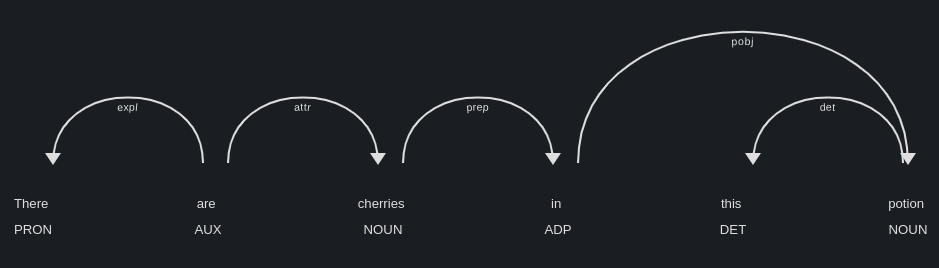
\includegraphics[scale=0.45]{Images/imgSpacy.png}
    \caption{Dependency parsing con Spacy}
    \label{fig:Spacy}
\end{figure}
A partire dall'albero ottenuto con spacy andiamo a ricercare quattro caratteristiche della frase:
\begin{itemize}
    \item Se è una domanda;
    \item Se è utile: cioè se la frase contiene ingredienti (in caso di utilità/non utilità verrà processata diversamente come si vedrà in seguito);
    \item Se contiene le parole yes/no;
    \item La sua polarità, cioè se è una frase affermativa o negativa;
\end{itemize}
\subsection{Frasi interrogative}
Per verificare se la frase sia o meno una domanda usiamo il metodo check\_if\_question in cui semplicemente verifichiamo se è presente un punto interrogativo o se la frase inizia con specifiche parole come "is", "are", "does", "do", "how" ecc...
\subsection{Frasi utili}
La verifica dell'utilità di una frase avviene nel metodo check\_if\_useful, qui percorriamo tutta la frase e analizziamo le relazioni che coinvolgono parole utili: il primo passo consiste nell'analizzare se la frase contiene parole volgari, se non le contiene, si va avanti. La lista delle parole utili che cerchiamo all'interno di una frase è contenuta nella knowledge\_base e contiene tutti gli ingredienti. Se un ingrediente è formato da più parole come "valerian spring", "mistletoe berry" o  "standard ingredient" analizziamo l'albero delle dipendenze cercando delle specifiche relazioni tra parole per riconoscerli. Per gli ingredienti nelle pozioni analizzate abbiamo riconosciuto quattro tipologie diverse di relazioni tra le parole:
\begin{itemize}
    \item \textbf{amod}: modificatore aggettivale, per ingredienti del tipo \textit{"mistletoe berry"};
    \item \textbf{poss}: relazioni possessive, per ingredienti come \textit{"bicorn's horn"};
    \item \textbf{compound}: nomi composti, per catturare ingredienti come \textit{"lether river water"};
    \item \textbf{nsubj}: per i casi in cui l'ingrediente è il soggetto della frase ma non copre uno dei casi precedenti, quindi ingredienti formati da una sola parola come \textit{"chicken"}, \textit{"spiders"};
    \item \textbf{prep}: quando abbiamo frasi con \textit{"There are ..."}
    \item \textbf{acomp} e \textbf{attr}: per frasi base come \textit{"The first ingredient is Fluxweed"}, molto spesso quando l'ingrediente si trova dopo \textit{is} oppure \textit{are}.
\end{itemize}
Se una frase contiene una o più parole che soddisfano uno di questi casi la frase viene etichettata come \textbf{useful}

\subsection{Frasi yes/no e polarità}
Per alcune tipologie di domande che Piton porrà allo studente sarà richiesta una risposta di tipo yes/no per riconoscere queste frasi il metodo \texttt{check\_yesno} verifica se la frase inizia con yes o con no o se non contiene affatto una di queste parole, si vedrà in seguito come reagirà Piton.
Per la polarità invece analizziamo l'albero delle dipendenze, riconosciamo polarità negativa se:
\begin{itemize}
    \item[i)] l'etichetta morph indica "Polarity=Neg";
    \item[ii)] l'etichetta dep indica "neg";
    \item[iii)] c'è un "no" che precede gli ingredienti per frasi del tipo \textit{"There are no cherries in this potion"}.
\end{itemize}
Diversamente la polarità sarà positiva
\subsection{Esempio di analisi di una frase}
Si mostra ora un esempio di analisi di una frase.
\begin{lstlisting}
  strin = PhraseAnalisys("There are cheries in this potion")
  pprint(strin.phrase)
  pprint(strin.dependency_tree())
  print(f"Is useful: {strin.check_if_useful()}")
  print(f"Polarity: {strin.check_polarity()}")
  print(f"Is question: {strin.check_if_question()}")
\end{lstlisting}
In questo esempio è stato volutamente commesso un errore di battitura sull'ingrediente cherries per dimostrare il funzionamento della correzione automatica dei refusi citata all'inizio.
\newline
\newline
Output:
\begin{lstlisting}
  'there are cherries in this potion '

  {'are': ('ROOT', 'are'),
   'cherries': ('attr', 'are'),
   'in': ('prep', 'cherries'),
   'potion': ('pobj', 'in'),
   'there': ('expl', 'are'),
   'this': ('det', 'potion')}

  Is useful: True
  Polarity: True
  Is question: False
\end{lstlisting}

Come ci aspettiamo l'analizzatore vede e corregge l'errore, riconosce la presenza dell'ingrediente, che non si tratta di una domanda è che la polarità è positiva.